% TeX eps-loader file generated by stoch_simul.m (Dynare).
% 14-May-2020 17:45:28
 
\begin{figure}[H]
\psfrag{log_y}[1][][0.5][0]{${\log(y)}$}
\psfrag{log_k}[1][][0.5][0]{${\log(k)}$}
\psfrag{log_c}[1][][0.5][0]{${\log(c)}$}
\psfrag{log_l}[1][][0.5][0]{${\log(l)}$}
\psfrag{log_w}[1][][0.5][0]{${\log(w)}$}
\psfrag{r}[1][][0.5][0]{${r}$}
\psfrag{A}[1][][0.5][0]{${A}$}
\centering 
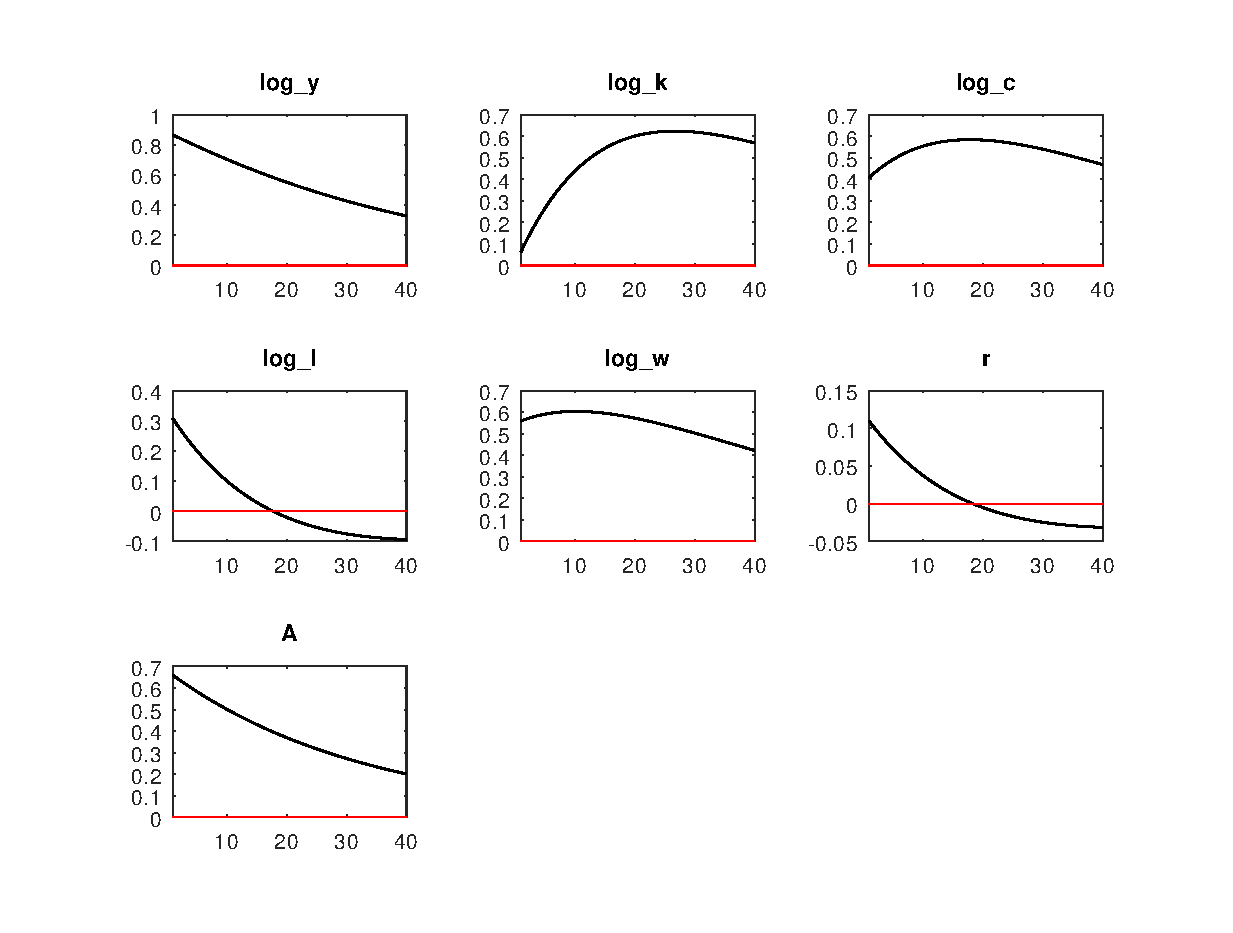
\includegraphics[width=0.80\textwidth]{RBCp_IRF_eps_A}
\caption{Impulse response functions (orthogonalized shock to ${\varepsilon_A}$).}
\label{Fig:IRF:eps_A}
\end{figure}
 
\begin{figure}[H]
\psfrag{log_y}[1][][0.5][0]{${\log(y)}$}
\psfrag{log_k}[1][][0.5][0]{${\log(k)}$}
\psfrag{log_c}[1][][0.5][0]{${\log(c)}$}
\psfrag{log_l}[1][][0.5][0]{${\log(l)}$}
\psfrag{log_w}[1][][0.5][0]{${\log(w)}$}
\psfrag{r}[1][][0.5][0]{${r}$}
\psfrag{ghat}[1][][0.5][0]{${\hat g}$}
\centering 
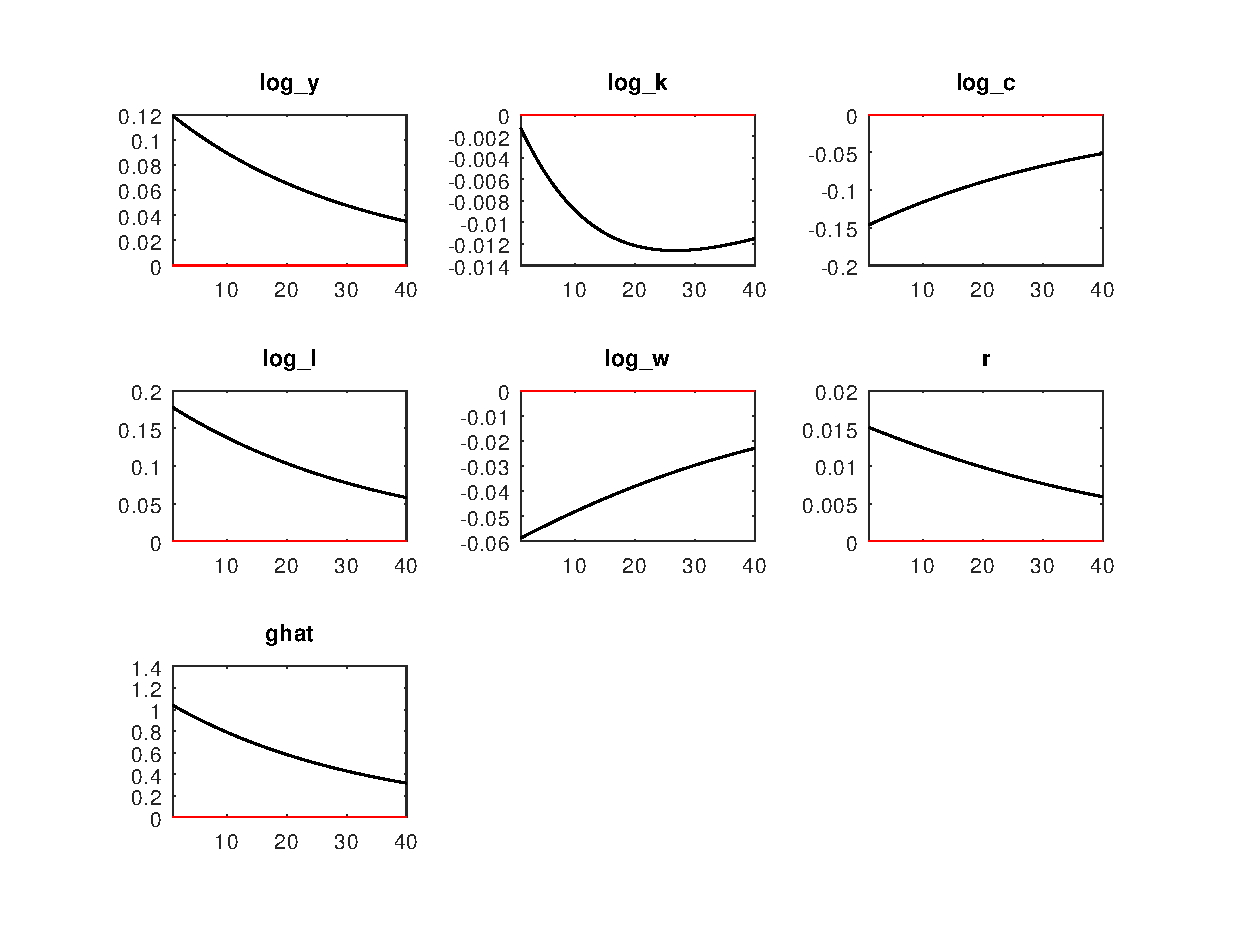
\includegraphics[width=0.80\textwidth]{RBCp_IRF_eps_g}
\caption{Impulse response functions (orthogonalized shock to ${\varepsilon_g}$).}
\label{Fig:IRF:eps_g}
\end{figure}
 
 
% End Of TeX file. 
